\documentclass[10pt]{article}
\usepackage[utf8]{inputenc}
\usepackage[T1]{fontenc}
\usepackage{amsmath}
\usepackage{amsfonts}
\usepackage{amssymb}
\usepackage[version=4]{mhchem}
\usepackage{stmaryrd}
\usepackage{graphicx}
\usepackage[export]{adjustbox}
\graphicspath{ {./images/} }
\usepackage{caption}

\author{Yonatan Sivan ${ }^{*, \dagger}$ and Yonatan Dubi ${ }^{\ddagger}$\\
† School of Electrical and Computer Engineering, Ben-Gurion University of the Negev, Israel\\
‡ Department of Chemistry, Ben-Gurion University of the Negev, Israel\\
E-mail: sivanyon@bgu.ac.il}
\date{}


\DeclareUnicodeCharacter{2020}{\ifmmode\dagger\else{$\dagger$}\fi}
\DeclareUnicodeCharacter{2021}{\ifmmode\ddagger\else{$\ddagger$}\fi}

\begin{document}
\maketitle
\captionsetup{singlelinecheck=false}
\section*{Supporting Information:}
\section*{Theory of "Hot" Photoluminescence from Drude}
\section*{Metals}


\section*{S1 A Fermi golden rule formulation of the field distribution due to light emission from metals}
In the context of nano-plasmonics, there is usually interest in the relative change of the total rate of photon emission due to the presence of the metal NP (compared to the case in which the NP is absent); this makes determination of the total field unnecessary.

In contrast, in the study of "hot" PL we are interested in the absolute number of emitted photons. We are also interested to obtan complete expression for the emitted electric field; this can enable a comparison of the scattering and emission cross-sections, or the emitted near-field with the absorption cross-section.

As a result, it is required to account for the emission rate of each of the modes in order to be able to determine the complete distribution of the electric field (i.e., both in the nearfield and far-field. In order to do that, we combine the Fermi golden rule formulation as presented in Ref. [S1] (a QED derivation for an emitter with a discrete energy spectrum\\
and arbitrary LDOPS) with that of Ref. S2 (a semi-classical derivation for systems with a continuous energy spectrum and free space LDOPS). For an electron in an initial state $\mathcal{E}_{i}$, the spontaneous emission rate is given by


\begin{equation*}
\left.R^{e m, i}(\vec{r}, \omega)=\frac{2 \pi}{\hbar} \sum_{f}|\langle f| \mathcal{H}(\vec{r}, \omega)| i\right\rangle\left.\right|^{2} f\left(\mathcal{E}_{i}\right)\left[1-f\left(\mathcal{E}_{f}\right)\right] \delta\left(\mathcal{E}_{f}-\mathcal{E}_{i}+\hbar \omega\right) \tag{S1}
\end{equation*}


where $\langle f|$ is the final quantum state of the whole system (not to be confused with $f$, the (non-equilibrium) electron distribution function) - it includes both the final electronic state, as well as the emitted photon state (i.e., its frequency $\omega$ and modal indices $n, l, m$; notation associated with other properties, such as polarization, wavevector, is suppressed); in addition, $\mathcal{H} \equiv \hat{\mu} \cdot \hat{\vec{E}}(\vec{r}, \omega)$ is the electric dipole operator, with $\hat{\vec{E}}(\vec{r}, \omega)$ being the emitted (only!) electric field and $\hat{\mu} \sim \vec{\mu}\left(\mathcal{E}_{i}, \mathcal{E}_{f}\right) \sim q_{e}\langle f| \hat{\mu}|i\rangle$ the transition dipole moment operator.

Importantly, we emphasize that for metal emission, one should replace $R^{e m, i}$, the number of photons emitted per unit time (in Hz ) at a specific frequency S 1 , by $\Gamma^{e m, i} d \omega$ which is the number of photons emitted per unit time and unit frequency (hence, unitless) $\stackrel{\mathrm{S} 2}{\text {; this is the }}$ quantity which is experimentally measured.

As shown in Eq. (8.98) of Ref. S1, it is convenient to rewrite the emitted field as a sum of the individual emitted and absorbed photon modes (in a standard second quantization fashion). In this case, the bra-ket term simplifies to


\begin{equation*}
\langle f| \vec{\mu} \cdot \hat{\vec{E}}\left(\vec{r}, \omega_{q}\right)|i\rangle=\vec{\mu} \cdot \sum_{q} \hat{\vec{E}}_{q}^{*}(\vec{r}, \omega) e^{i \omega_{q} t}\left\langle\mathcal{E}_{f}, 1_{\omega_{q^{\prime}}} \mid \mathcal{E}_{f}, 1_{\omega_{q}}\right\rangle \tag{S2}
\end{equation*}


and a similar expression for its Hermitian conjugate; here, $\hat{\vec{E}}_{q}(\vec{r}, \omega)$ is the $q$ 'th mode of the NP; the notation of the photon frequency was modified to $\omega_{q}$ where $q$ represents a general set of "quantum" numbers (e.g., $n, l$ and $m$ for 3D particles). Thus, Eq. (S1) can be written\\
as

$$
\begin{aligned}
R^{e m, i}(\vec{r}, \omega)= & \sum_{q} R_{q}^{e m, i} \\
R_{q}^{e m, i}= & \frac{2 \pi}{\hbar}\left[\left(\hat{n}_{\mu} \cdot \sum_{q^{\prime \prime}} \hat{\vec{E}}_{q^{\prime \prime}}\left\langle\mathcal{E}_{f}, 1_{\omega_{q^{\prime \prime}}} \mid \mathcal{E}_{f}, 1_{\omega_{q^{\prime}}}\right\rangle\right)\left(\sum_{q^{\prime}} \hat{\vec{E}}_{q^{\prime}}^{*}\left\langle\mathcal{E}_{f}, 1_{\omega_{q^{\prime}}} \mid \mathcal{E}_{f}, 1_{\omega_{q}}\right\rangle \cdot \hat{n}_{\mu}\right)\right] \times \\
& \int\left|\vec{\mu}\left(\mathcal{E}_{f}, \mathcal{E}_{i}\right)\right|^{2} e^{i\left(\omega_{q}-\omega_{q^{\prime \prime}}\right) t} f\left(\mathcal{E}_{i}\right)\left[1-f\left(\mathcal{E}_{f}\right)\right] \delta\left(\mathcal{E}_{f}-\mathcal{E}_{i}+\hbar \omega_{q^{\prime}}\right) N_{e}\left(\mathcal{E}_{f}\right) d \mathcal{E}_{f}
\end{aligned}
$$

where the factor $|\vec{\mu}|^{2}$ was extracted and the unit vector $\hat{n}_{\mu}$ representing its directionality remained. We also split $\sum_{f}$ to $\sum_{q} \int N_{e}\left(\mathcal{E}_{f}\right) d \mathcal{E}_{f}$ where $N_{e}$ is the number of electrons per unit of energy. Assuming that the NP is more than a few nm in size, and that electron DOS is spatially-uniform, $N_{e}$ is related to the local density of states $\rho_{e}$ simply via $N_{e}(\mathcal{E})=\rho_{e}(\mathcal{E}) V_{N P}$ where $\rho_{e}=\frac{3 n_{e}}{2 \mathcal{E}_{F}} \sqrt{\frac{\mathcal{E}}{\mathcal{E}_{F}}}$.

Photon mode orthogonality dictates that $\omega_{q}=\omega_{q^{\prime}}=\omega_{q^{\prime \prime}} \equiv \omega$ so that $q^{\prime \prime}=q^{\prime}=q$ in which case the bra-ket terms become unity. Thus,


\begin{equation*}
R^{e m, i}(\vec{r}, \omega)=\frac{2 \pi}{\hbar} \sum_{q}\left(\hat{n}_{\mu} \cdot \hat{\vec{E}}_{q}\right)\left(\hat{\vec{E}}_{q}^{*} \cdot \hat{n}_{\mu}\right) \int\left|\vec{\mu}\left(\mathcal{E}_{f}, \mathcal{E}_{i}\right)\right|^{2} N_{e}\left(\mathcal{E}_{f}\right) f\left(\mathcal{E}_{i}\right)\left(1-f\left(\mathcal{E}_{f}\right)\right) \delta\left(\mathcal{E}_{f}-\mathcal{E}_{i}+\hbar \omega\right) d \mathcal{E}_{f} \tag{S3}
\end{equation*}


Eq. (S3) shows that in the current formulation, the exact properties of the electron wavefunctions appear via the dipole transition moment $\vec{\mu}$ and via the energy conservation within the electronic band structure.

The sum over modes can now converted to the LDOPS via the (canonical) normalization of the modes (see Eq. (4.99) of Ref. [S3]), namely,


\begin{equation*}
\rho_{p h o t}(\omega) \equiv 3 \sum_{n, l, m}\left(\hat{n}_{\mu} \cdot \hat{\vec{u}}_{q}\right)\left(\hat{\vec{u}}_{q}^{*} \cdot \hat{n}_{\mu}\right) \delta\left(\left(\mathcal{E}_{f}-\mathcal{E}_{i}\right) / \hbar+\omega\right), \quad \hat{\vec{E}}_{q}(\vec{r})=\sqrt{\frac{\hbar \omega}{2 \epsilon_{0}}} \hat{\vec{u}}_{q}(\vec{r}) \tag{S4}
\end{equation*}


At this point, standard derivations for a quantum 2-level emitter (e.g., in Ref. [S1,S4])\\
consider the extreme non-equilibrium scenario (complete population inversion) in which $f(1- f) \approx 1$. In this case, the overall emission rate is given by


\begin{equation*}
R^{e m, i}(\vec{r}, \omega)=\frac{\pi \omega}{3 \epsilon_{0}}|\vec{\mu}|^{2} \rho_{p h o t}(\omega) N_{e}\left(\mathcal{E}_{f}\right) d \omega \tag{S5}
\end{equation*}


For free space, $\rho_{\text {phot }}=\omega^{2} / \pi^{2} c^{3}$, so that


\begin{equation*}
\Gamma^{e m, i}(\vec{r}, \omega)=\frac{\omega^{3}}{3 \pi \epsilon_{0} c^{3}}|\vec{\mu}|^{2} N_{e}\left(\mathcal{E}_{f}\right) \tag{S6}
\end{equation*}


In the general case, however, the occupation $f$ is incomplete ( $<1$ ), and the electronic system is characterized by a continuum of states. Thus, we proceed differently, namely, we perform the integration over the final electron state energy in (S3) and obtain the total emission rate at a given frequency by integrating over the initial electron energy (while including the proper number of electron states again). Thus,


\begin{align*}
R^{e m}(\vec{r}, \omega) & =\sum_{q} R_{q}^{e m}(\vec{r}, \omega)  \tag{S7}\\
R_{q}^{e m}(\vec{r}, \omega) & =\int N_{e}\left(\mathcal{E}_{i}\right) R_{q}^{e m, i}(\vec{r}, \omega) d \mathcal{E}_{i} \\
& =\frac{2 \pi V_{N P}^{2}}{\hbar}\left(\hat{n}_{\mu} \cdot \hat{\vec{E}}_{q}(\vec{r})\right)\left(\hat{\vec{E}}_{q}^{*}(\vec{r}) \cdot \hat{n}_{\mu}\right) \int\left|\vec{\mu}\left(\mathcal{E}_{i}, \mathcal{E}_{i}+\hbar \omega\right)\right|^{2} \rho_{J}\left(\mathcal{E}_{i}, \mathcal{E}_{i}+\hbar \omega\right) d \mathcal{E}_{i}
\end{align*}


where


\begin{equation*}
\rho_{J}(\mathcal{E}, \mathcal{E}+\hbar \omega)=\left[f(\mathcal{E}+\hbar \omega) \rho_{e}(\mathcal{E}+\hbar \omega)\right]\left[\left(1-f(\mathcal{E}) \rho_{e}(\mathcal{E})\right]\right. \tag{S8}
\end{equation*}


The (canonical) normalization (S4) allows us to write the above relations also as


\begin{align*}
R^{e m}(\vec{r}, \omega) & =\frac{2 \pi V_{N P}^{2}}{\hbar} \frac{\hbar \omega}{2 \epsilon_{0}} \sum_{q}\left(\hat{n}_{\mu} \cdot \hat{\vec{u}}_{q}\right)\left(\hat{\vec{u}}_{q}^{*} \cdot \hat{n}_{\mu}\right) \int|\vec{\mu}(\mathcal{E}, \mathcal{E}+\hbar \omega)|^{2} \rho_{J}(\mathcal{E}, \mathcal{E}+\hbar \omega) d \mathcal{E} \\
& =\frac{\pi \omega V_{N P}^{2}}{\epsilon_{0}} g_{p h o t}(\vec{r}, \omega) \int|\vec{\mu}(\mathcal{E}, \mathcal{E}+\hbar \omega)|^{2} \rho_{J}(\mathcal{E}, \mathcal{E}+\hbar \omega) d \mathcal{E} \tag{S9}
\end{align*}


where $g_{\text {phot }}$ (the number of states per unit volume in interval $\omega$ to $\omega+d \omega$, aka degeneracy) is defined via $\rho_{\text {phot }}(\vec{r}, \omega) d \omega \equiv g_{\text {phot }}(\vec{r}, \omega) .{ }^{\text {S3 }}$ In these terms, Eq. (S9) becomes


\begin{equation*}
\Gamma^{e m}(\vec{r}, \omega)=\frac{\pi \omega V_{N P}^{2}}{\epsilon_{0}} \rho_{p h o t}(\vec{r}, \omega) \int|\vec{\mu}(\mathcal{E}, \mathcal{E}+\hbar \omega)|^{2} \rho_{J}(\mathcal{E}, \mathcal{E}+\hbar \omega) d \mathcal{E} \tag{S10}
\end{equation*}


Note that the product of $V_{N P}^{2}$ and $\rho_{e}^{2}$ removes the volume dependence and yields a quadratic scaling with the electron number. This arises from the double summation over the initial and final energies.

\section*{S2 The non-equilibrium electron distribution}
We rely on the semi-quantum formulation derived for the determination of the non-equilibrium electron distribution in metals and described comprehensively in Ref. S5, S6. This formulation included the dominant effects of photon absorption, $e-e$ collisions and $e-p h$ collisions. Specifically, it relied on the following generic Boltzmann equation,


\begin{equation*}
\frac{\partial f\left(\mathcal{E} ; T_{e}, T_{p h}\right)}{\partial t}=\underbrace{\left(\frac{\partial f}{\partial t}\right)}_{\text {photon absorption }}+\underbrace{\left(\frac{\partial f}{\partial t}\right)}_{e-\text { ph collisions }}+\underbrace{\left(\frac{\partial f}{\partial t}\right)}_{e-e \text { collisions }} \tag{S11}
\end{equation*}


where $f$ is the electron distribution function at an energy $\mathcal{E}$, electron temperature $T_{e}$ and phonon temperature $T_{p h}$, representing the population probability of electrons in a system characterized by a continuum of states within the conduction band. The first term on the right-hand-side (RHS) of Eq. (S11) describes excitation of conduction electrons due to photon absorption, see SI Section IA in Ref. [S5] for its explicit form. The second term on the RHS of Eq. (S11) describes energy relaxation due to collisions between electrons and phonons, see SI Section IB in Ref. [S5] for its explicit form. The third term on the RHS of Eq. (S11) represents the thermalization induced by $e-e$ collisions, i.e., the convergence of\\
the non-thermal population into the thermalized Fermi-Dirac distribution, given by


\begin{equation*}
f^{T}\left(\mathcal{E} ; T_{e}\right)=\left(1+e^{\left(\mathcal{E}-\mathcal{E}_{F}\right) / k_{B} T_{e}}\right)^{-1} \tag{S12}
\end{equation*}


where $k_{B}$ is the Boltzmann constant. Its explicit form, within the Relaxation Time Approximation is given in SI Section IC in Ref. S5].

Note that this formulation ignores the quantum description of plasmon generation and decay, hence, it is valid for particles more than a few nm in size such that electron energy quantization effects would be negligible (as shown in Ref. S7). Since we operate in energy space, momentum conservation in $e-e$ interactions is ignored. This causes an inaccuracy which is expected to be small because it is mostly relevant for the very few high energy non-thermal electrons. This approach is, however, customary when treating nanoparticles.

In order to get a quantitatively valid distribution, the Boltzmann equation (S11) has to be complemented with a (even phenomenological) equation for the phonon energy/temperature, and energy conservation in the whole system (consisting of photons, electrons, phonons, and the environment) must be enforced.

\section*{S3 The joint density of of pair states for illuminated metals}
Knowing the non-equilibrium electron distribution allows us to plot the population-weighted joint density of pair states (JDOPS (2)). In Fig. S 1 we plot the JDOPS corresponding to several emission frequencies for both the non-thermal distribution, as well as its thermal counterpart. Already a-priori, it is trivial to appreciate that the (nearly-)flat part of the integrand (i.e., the "hot electron" shoulder) would cause the ("hot", or non-thermal) JDOPS (red) to be higher with respect to the thermal case (black). As a result, the emission is expected to be stronger than the thermal case, hence, to decay slower with the frequency.

This already implies that any attempt to associate a temperature with this slope is destined to yield a value higher than the actual electron temperature.

Plotting the JDOPS (see Fig. S1) indeed reveals quantitative differences between the thermal and the non-thermal cases; interestingly, we also observe significant qualitative differences. First, while in the thermal case the integrand has a flat top profile from which the major contribution originates, one can see that in the non-thermal case (Fig. S1) the integrands have a double peak profile (Note that the approximate symmetry observed now in Fig. S1 will be somewhat distorted once the eDOS is accounted for). More specifically, for the SE ( $\omega<\omega_{L}$ ), one can appreciate that the region that contributes the most to the total emission is the "hot" electron shoulder (see red-shaded regions). This explains why in this spectral regime the magnitude of the integrand (hence, the emission) is weakly-dependent on the emission frequency (compare Figs. S1 (a) \& (b)); since the shoulder height is independent of $T_{e}$ (see Eq. (3)), this also shows that the SE should be temperature-insensitive and that it should scale as $\left|\hat{E}_{L}\right|^{2}$. This prediction is in agreement with the experimental observations in Ref. S8 S11 and our analytic result (8).

In contrast to the SE and in partial similarity to the BB emission, the aSE originates from the product of the thermal regime of the electron distribution (immediately beyond the Fermi energy) and the regime just beyond the edge of the first shoulder (see Figs. S1 (c)-(d)); as explained in the main text, this part of the electron distribution is a "copy" of the thermal regime of the electron distribution around the Fermi energy due to two uncorrelated photon absorption events. Therefore, unlike the SE, the aSE grows with the temperature, as reported for the first time in Ref. S9, S10 and has a non-trivial polynomial dependence on $\left|\hat{E}_{L}\right|^{2}$, see Fig. 3(b). In addition, when the emission frequency grows, the overlap of $f(\mathcal{E}+\hbar \omega)$ and $1- f(\mathcal{E})$ occurs at lower occupation probabilities such that the overall aSE decays exponentially with the emission frequency (like in the $\mathrm{BB}(/ \mathrm{PL})$ case, compare Fig. S1(c) \& (d)). This role of the thermal part of the distribution explains why qualitative predictions about the emission curves may have been obtained without knowing the actual non-equilibrium distribution, but\\[0pt]
rather, by assuming the distribution is purely thermal (as e.g., in Ref. [S12-S14]); this also motivated the underlying assumption of the thermometry protocols that emerged recently. As we will show in a consequent paper, this assumption turns out to be somewhat crude.

\begin{figure}[h]
\begin{center}
  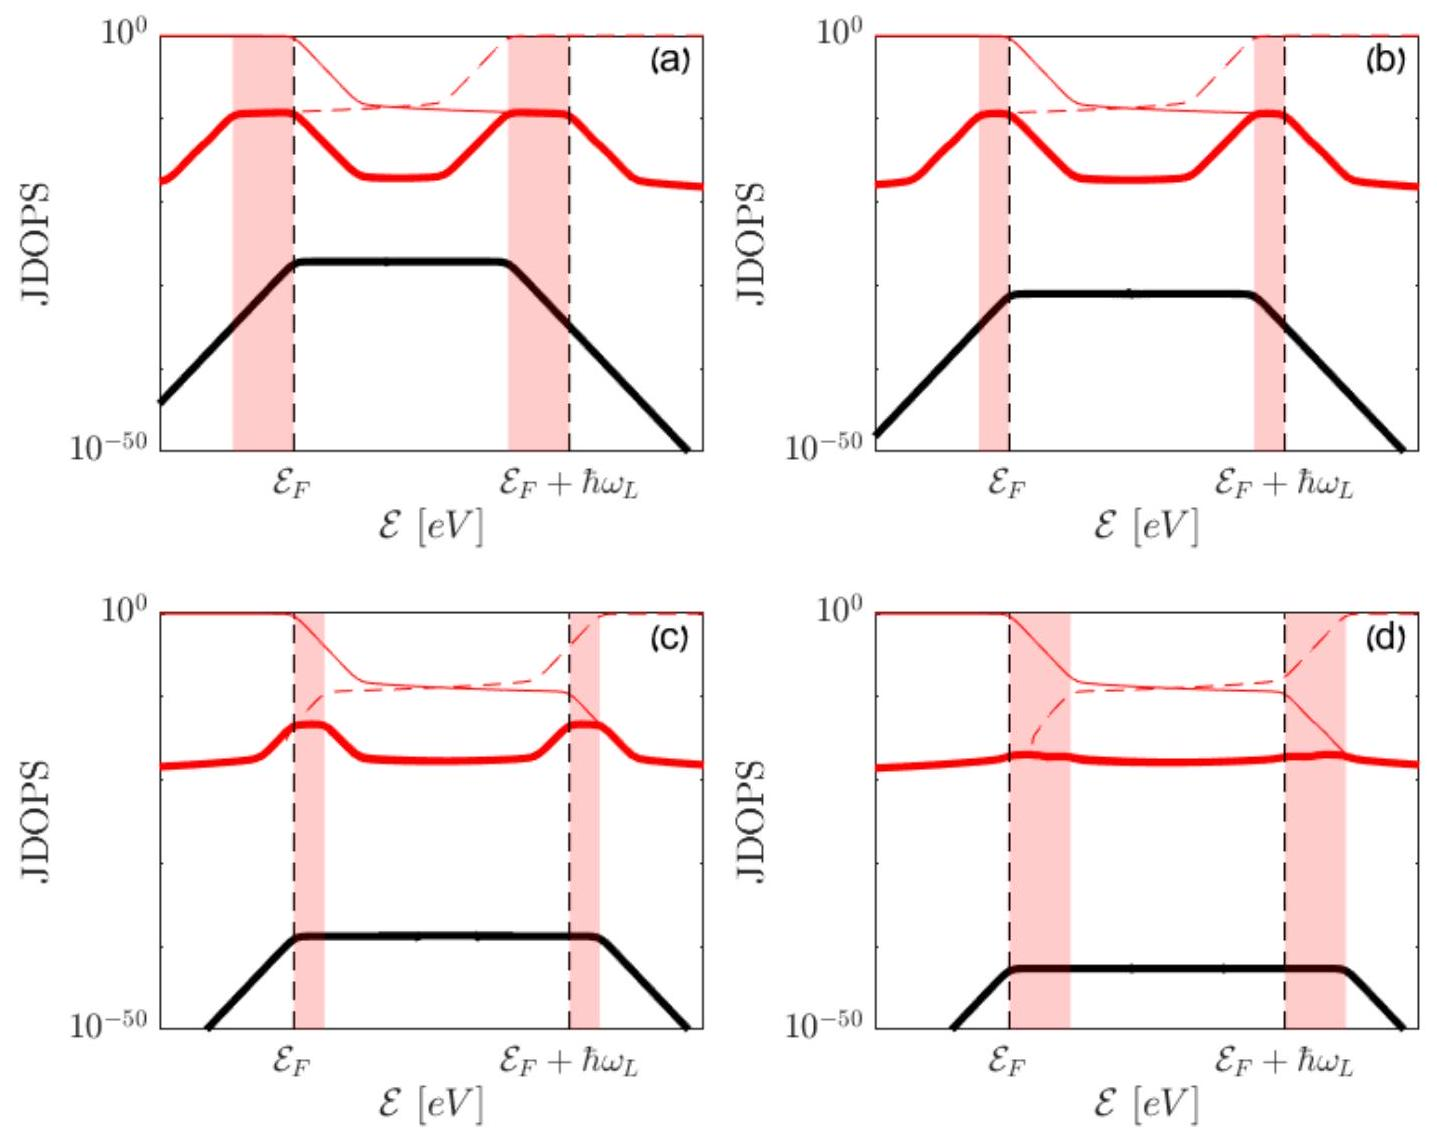
\includegraphics[alt={},max width=\textwidth]{865cfde5-08a8-45cc-b3b2-2cc5e58acbb9-08_1142_1437_569_302}
\captionsetup{labelformat=empty}
\caption{Figure S1: (Color online) (a)-(d) The population-weighted density of pair states (the integrand in Eq. (1), thick red solid) for $\hbar \omega=\hbar \omega_{L}-0.5 \mathrm{eV}, \hbar \omega_{L}-0.2 \mathrm{eV}, \hbar \omega_{L}+0.15 \mathrm{eV}, \hbar \omega_{L}+0.3 \mathrm{eV}$, respectively; the population $f(\mathcal{E})$ (red solid) is shown again, along with the corresponding hole population $1-f(\mathcal{E}-\hbar \omega)$ (red dashed). The data cutoff at low energies is a numerical issue. Regions from which the main contribution to the emission are marked in shaded color.}
\end{center}
\end{figure}

\section*{References}
(S1) Novotny, L.; Hecht, B. Principles of Nano-Optics; Cambridge University Press, Cambridge, 2006.\\
(S2) Bebb, H. B.; Williams, E. W. In Chapter 4 Photoluminescence I: Theory; Willardson, R. K., Beer, A. C., Eds.; Semiconductors and Semimetals; Elsevier, New York and London, 1972; Vol. 8; pp 181-320.\\
(S3) Grynberg, G.; Aspect, A.; Fabre, C. Introduction to Quantum Optics: From the Semiclassical Approach to Quantized Light; Cambridge University Press, Cambridge, 2010.\\
(S4) Cohen-Tannoudji, C.; Diu, B.; Laloë, F. Quantum Mechanics; John Wiley \& sons, Paris, France, 1977.\\
(S5) Dubi, Y.; Sivan, Y. "Hot Electrons" in Metallic Nanostructures - Non-Thermal Carriers or Heating? Light: Sci. Appl. 2019, 8, 89.\\
(S6) Sivan, Y.; Un, I. W.; Dubi, Y. Assistance of Plasmonic Nanostructures to Photocatalysis - Just a Regular Heat Source. Faraday Discuss. 2019, 214, 215-233.\\
(S7) Besteiro, L. V.; Kong, X.-T.; Wang, Z.; Hartland, G.; Govorov, A. O. Understanding Hot-Electron Generation and Plasmon Relaxation in Metal Nanocrystals: Quantum and Classical Mechanisms. ACS Photonics 2017, 4, 2759-2781.\\
(S8) Beversluis, M.; Bouhelier, A.; Novotny, L. Continuum Generation from Single Gold Nanostructures through Near-Field Mediated Intraband Transitions. Phys. Rev. B 2003, 68, 115433.\\
(S9) Hugall, J. T.; Baumberg, J. J. Demonstrating Photoluminescence from Au is Electronic Inelastic Light Scattering of a Plasmonic Metal: The Origin of SERS Backgrounds. Nano Lett. 2015, 15, 2600-2604.\\
(S10) Huang, J.; Wang, W.; Murphy, C. J.; Cahill, D. G. Resonant Secondary Light Emission from Plasmonic Au Nanostructures at High Electron Temperatures Created by PulsedLaser Excitation. Proc. Nat. Acad. Sci. U.S.A 2014, 111, 906-911.\\
(S11) Carattino, A.; Caldarola, M.; Orrit, M. Gold Nanoparticles as Absolute NanoThermometers. Nano Lett. 2017, 18, 874-880.\\
(S12) Boyd, G. T.; Yu, Z. H.; Shen, Y. R. Photoinduced Luminescence from the Noble Metals and Its Enhancement on Roughened Surfaces. Phys. Rev. B 1986, 33, 7923.\\
(S13) Otto, A.; Akemann, W.; Pucci, A. Normal Bands in Surface-Enhanced Raman Scattering (SERS) and Their Relation to the Electron-Hole Pair Excitation Background in SERS. Isr. J. Chem. 2006, 46, 307-315.\\
(S14) Shahbazyan, T. V. Theory of Plasmon-Enhanced Metal Photoluminescence. Nano Lett. 2013, 13, 194-198.


\end{document}